\documentclass[10pt,twocolumn]{article}
\usepackage{latexsym,amssymb,enumerate,amsmath,epsfig,amsthm}
\usepackage[margin=1in]{geometry}
\usepackage{setspace,color}
\usepackage{graphicx}
\graphicspath{{figures/}}
\usepackage{subfigure}
\usepackage[english]{babel}
\usepackage[table,xcdraw]{xcolor}
\usepackage[utf8]{inputenc}
\usepackage{amsmath}
\usepackage{graphicx}
\usepackage[colorinlistoftodos]{todonotes}
\usepackage{geometry}
\usepackage{caption}
\usepackage{url}
\usepackage{array}
\usepackage[toc,page]{appendix}
\usepackage{booktabs}
\usepackage{float}
\usepackage{hyperref}
\usepackage{xcolor}
\usepackage{tabularx}
\usepackage{cite}
\hypersetup{
 colorlinks,
 linkcolor={red!50!black},
 citecolor={blue!50!black},
 urlcolor={blue!80!black}
}
\DeclareMathOperator*{\argmax}{arg\,max}
\usepackage{listings}
\usepackage{xcolor}

\lstset{
 basicstyle=\ttfamily\footnotesize,
 breaklines=true,
 frame=single,
 columns=fullflexible,
 backgroundcolor=\color{gray!10},
 keywordstyle=\color{blue},
 commentstyle=\color{gray},
 stringstyle=\color{red!70!black},
 showstringspaces=false,
 tabsize=2
}


\begin{document}

\title{Evaluating Treatment Options for Chronic Kidney Disease Stage 5 using a Markov Decision Process}
\author{
Brian Bowers, undergraduate at Loyola Marymount University}

\twocolumn[
  \begin{@twocolumnfalse}
    \date{May 9, 2025}
    \maketitle
    \begin{abstract} 

Chronic Kidney Disease (CKD) roughly affects 1 in 7 United States adults \cite{cdc}, many of whom may not know that they currently have CKD. The disease progresses slowly, eventually reaching a state where the kidneys can no longer properly filter waste and other fluids from your blood. Since many adults do not realize they have CKD the disease can progress to a late stage before a diagnosis is made. Once this late stage is reached, more serious treatment options are required, which include conservative care, dialysis, and transplant. In this paper, we will model the progression of Chronic Kidney Disease Stage 5 using a Markov Decision Process (MDP). We will solve the MDP using value iteration to get the optimal policy, which will allow us to determine the best treatment choices. Using the same model, we will conduct a Monte Carlo Simulation to determine the optimal treatment and the average lifespan, quality of life, and quality-adjusted life years, for each of the treatments. Finally, we will compare the results of these two different methods. \\
    \end{abstract}
  \end{@twocolumnfalse}
]

% ------------------------------------------------------------------------------------------
%    Background Section
% ------------------------------------------------------------------------------------------

\section{Background}
Ideally, patients with CKD are initially diagnosed in Stage 1. Then over the next few years, they will slowly progress through states, until they reach CKD Stage 5. However, many people with CKD go undiagnosed, as the symptoms can be hard to detect. To determine whether a patient has CKD two tests are used. The first test is called eGFR and it measures the creatinine levels in the blood and determines how well the kidneys are filtering waste. The second test, uACR, is a urine test that measures the ratio between albumin and creatinine \cite{Chronic}. Typically, patients in the lower stages of CKD are treated through medication and lifestyle changes. The medication is usually for treating the underlying cause of CKD, which can help slow down the progression of the disease \cite{Prescribing}. Lifestyle changes consist of individualized diets, exercise, drinking less alcohol, etc. Generally, these treatments can be grouped together as Conservative Care (CC), which are treatments that do not replace the functions of the kidney \cite{Treatments}.

Dialysis is one of the treatments for late-stage CKD. During dialysis a patient's blood is removed from their body, cleaned with a machine that filters waste and excess fluids, and then pumps the blood back into the body. This helps to manage the symptoms of CKD and keep the patient alive, but it does not treat the disease \cite{survival}. Patients who decide to undergo dialysis also have the option of getting surgery to help lower the risks of dialysis. During this procedure, called a Fistula, a vein and an artery are connected together, usually in the forearm. This helps to ensure that the blood is pumped in and out of the body more easily, with fewer side effects \cite{Chronic}.

The last treatment is a transplant. To get a donor kidney, the patient must first be added to a list and must be eligible, by passing a series of requirements. Once a matching kidney is available, the patient can undergo transplant surgery. If the transplant is successful, the donated kidney will replace some of the functions of the failing kidney. However, it is generally still not a cure, and depending on the underlying disease their kidneys will continue to decrease in function. Furthermore, the patient has a chance of the operation failing or the kidney being rejected by the body. To try to prevent rejection patients are usually given immunosuppressants \cite{Chronic}.

Despite being on a treatment plan, there are several complications that can occur. While there are many of these, one of the most important ones is a stroke. Strokes occur when the blood flow to the brain is disrupted, and are more common in people with CKD. Strokes can result in death, varying degrees of disability, and loss of brain function, or they can be minor. Another common condition in patients is Myocardial Infarction (MI), which is when the heart muscles die due to not receiving enough blood \cite{long-term}. This can also result in death, but if the patient survives they are generally left with Congestive Heart Failure (CHF), which is when the heart is unable to pump blood effectively \cite{ckdmodel}.

Patients who have CKD must decide which treatments to undergo. To help them decide the benefits of each of the treatments, the patients need to know the effectiveness, benefits, and disadvantages of each treatment. To measure the effectiveness of a treatment, there are multiple factors that need to be considered. The first is the number of years a treatment will prolong a patient's life span. However, just increasing the lifespan is not always a beneficial thing, as a patient could be living in extreme pain or living just due to external devices. To address this there is an objective measure called quality of life (QoL) that can be determined. It is measured on a scale from dead (0.0) to full health (1.0). Combining these two measures allows us to calculate a patient's quality-adjusted life years (QALY) \cite{ckdmodel}, a measure that takes into account both lifespan and QoL.


% ------------------------------------------------------------------------------------------
%    Methods
% ------------------------------------------------------------------------------------------

\section{Methods}
\subsection{Markov Decision Process}
In this paper, we will model CKD using a Markov Decision Process (MDP). MDPs are useful for modeling sequential decisions in a stochastic environment \cite{ai}, which makes them useful for modeling chronic disease progression and treatment options. Specifically, CKD can represent a stochastic environment where there is a random chance that a patient will develop some condition, given the specific treatment option a patient chooses.

To use an MDP model we must first define the states, decisions, rewards, and transitions. Specifically, in an MDP, \(s_0\) is the initial state, which for our model is Chronic Kidney Disease Stage 5 (CKD5). We are assuming that a patient is currently in CKD5, meaning that they have very limited kidney function and must make decisions about which treatment to select. These decisions are modeled in the MDP as ACTIONS(\(s\)), which is the set of possible actions in each state. In our model, the patient has two actions or decisions that they need to make. The first decision is which treatment pathway they want to take. Their options are Conservative Care (CC), transplant, and dialysis. If the patient ever goes on dialysis, they have to make a decision between regular dialysis, with a catheter, and dialysis with a fistula. Each decision that a patient makes affects which next state they can go to and the probabilities of those states. The transitions between different states in the disease is defined by the transition model: \(P(s' | s, a)\), where \(s\) is the current state, \(s'\) is the next state, and \(a\) is the action. The transitions follow the Markovian property, where each next state depends only on the current state and not the history of previous states. Each state is given a utility value, a measure of the patient's QoL in that state, which in an MDP is expressed as \(U(s)\). From the utility function, a reward model \(R(s)\) can be defined. Finally, the solution to an MDP is a policy, which gives the best state to transition to given the current state. A policy is represented as \(\pi\), with \(\pi^*\) representing the optimal policy \cite{ai}.

By framing CKD stage 5 as an MDP we can determine what the best course of treatment is (between transplant, CC, and dialysis). In addition, for patients who either end up on dialysis after a transplant or choose dialysis, we will determine if it is better to get a fistula. Furthermore, our methods of solving the model will also allow us to determine the QoL of a patient, the expected lifespan, and the QALY of a patient, all depending on which actions they choose. This will allow us to effectively compare the effectiveness of each treatment option.

We will assume an MDP with an infinite horizon. This means that there is no fixed time limit, so therefore, theoretically a person could live forever. An infinite horizon means that the optimal action only depends on the current state, and therefore, the policy is said to be stationary because it doesn't depend on the current time step \cite{ai}. This does not mean that the sequence of states is always infinite, it just means there is a possibility of the model never-ending, which in this case is due to cycles within the model. In our model, we have a terminal state, which is death, and has a utility value of 0.0. As the time step approaches infinity, the model will likely have stopped in the absorbing death state. We also make the assumption that the MDP is fully observable, meaning that the patient has complete and accurate knowledge of their current health state, as well as is aware of all the possible treatment options for their condition.

\subsection{Parameters}
In Table \ref{tab:transit1} through Table \ref{tab:trans4} we define \(P(s' | s, a)\), the transitions from one state to another. The probabilities for the model are estimated from studies conducted on CKD. All the transition probabilities are the one-month probability of a patient moving to the state \(s'\) given the action \(a\) and state \(s\). This time frame is chosen because CKD is a slow-progressing disease, and patients can continue to live for years, especially on dialysis or after a transplant.

\begin{table}[ht]
  \centering
  \caption{Transition probabilities of treatment CC}
  \label{tab:transit1}
  \begin{tabularx}{\columnwidth}{X c c} 
      \toprule
 State \(\rightarrow\) Next State & Prob & Source \\ 
      \midrule
 CC \(\rightarrow\) Death & 0.09812 & \cite{survival}, solved \\
 CC \(\rightarrow\) Stroke & 0.006 & \cite{ckdmodel} \\
 CC \(\rightarrow\) MI & 0.00792 & \cite{ckdmodel} \\
 CC \(\rightarrow\) CC & 0.88796 & solved \\

 Stroke \(\rightarrow\) Disability & 0.33 & \cite{ckdmodel} \\
 Stroke \(\rightarrow\) Death & 0.2 & \cite{ckdmodel} \\
 Stroke \(\rightarrow\) CC & 0.47 & solved \\

 MI \(\rightarrow\) Death & 0.08 & \cite{ckdmodel} \\
 MI \(\rightarrow\) CHF & 0.05 & \cite{ckdmodel} \\
 MI \(\rightarrow\) CC & 0.87 & solved \\

 Disability \(\rightarrow\) CC & 1.0 & solved \\
 CHF \(\rightarrow\) CC & 1.0 & solved \\
      \bottomrule
  \end{tabularx}
\end{table}

Table \ref{tab:transit1} defines the probabilities \(P(s' | s, a)\) using studies conducted on CKD. We assume that the patient is in CKD5 and has decided to opt for conservative care. Here the probability of death is higher than in other states, which makes sense because the treatment option is not replacing the function of their kidneys. If a patient is in CKD5 and is not undergoing dialysis or a transplant, they generally will not live very long. The probability of death was given by \cite{survival}. They stated that the hazard rate of dialysis compared to CC was 0.47, meaning people on CC have a 2.13 times higher mortality rate. The mortality rate of our dialysis pathway was calculated using the Law of Total Probability and then multiplied by 2.13 to get the final value.

A patient undergoing CC has the risk of a stroke, leading to disability, or death. In addition, they also have the probability of developing an MI, leading to CHF or death. In Table \ref{tab:transit1}, solved means that some calculations were performed to get the probability, or it was determined from the model structure.

\begin{table}[ht]
  \centering
  \caption{Transition probabilities of treatment Transplant}
  \label{tab:trans2}
  \begin{tabularx}{\columnwidth}{X c c} 
      \toprule
 State \(\rightarrow\) Next State & Prob & Source \\ 
      \midrule
 Transplant \(\rightarrow\) Death & 0.012 & \cite{ckdmodel} \\
 Transplant \(\rightarrow\) Successful & 0.988 & solved \\
      
 Successful \(\rightarrow\) Dialysis & 0.0051 & \cite{ckdmodel} \\
 Successful \(\rightarrow\) MI & 0.0028 & \cite{ckdmodel}, solved \\
 Successful \(\rightarrow\) Death & 0.0031 & \cite{ckdmodel} \\
 Successful \(\rightarrow\) Stroke & 0.003 & \cite{ckdmodel} \\
 Successful \(\rightarrow\) Successful & 0.986 & solved \\
      
 Stroke \(\rightarrow\) Disability & 0.33 & \cite{ckdmodel} \\
 Stroke \(\rightarrow\) Death & 0.2 & \cite{ckdmodel} \\
 Stroke \(\rightarrow\) Successful & 0.47 & solved \\
      
 MI \(\rightarrow\) CHF & 0.05 & \cite{ckdmodel} \\
 MI \(\rightarrow\) Death & 0.08 & \cite{ckdmodel} \\
 MI \(\rightarrow\) Successful & 0.87 & solved \\
      
 CHF \(\rightarrow\) Successful & 1.0 & solved \\
 Disability \(\rightarrow\) Successful & 1.0 & solved \\  
      \bottomrule
  \end{tabularx}
\end{table}

Table \ref{tab:trans2} provides the transition probabilities given that the patient is in CKD5 and has chosen the treatment option transplant. There are two possible transitions from transplant, to death and to successful. Death means that the patient did not survive the transplant surgery, which is a low probability. Successful means that the surgery was completed. The model does not consider the possibility of the surgery failing, but the patient not dying.

If the transplant is successful there are three possible next states. First, there is a probability that the kidney will fail or be rejected within the first month. This model assumes that if the kidneys fail or are rejected, then the patient will go back onto dialysis, meaning they will transition to the dialysis action state. This is a slight simplification, as in this model we do not allow for the patient to have multiple transplants as multiple kidney transplants are rare. The next state a patient can transition to is stroke. The stroke can either result in death or disability. The probability of transition to stroke is based on the assumption that a patient who has a transplant will be in either CKD stage 2 or 3. The last transition is to MI, which can result in either death or CHF.

\begin{table}[ht]
  \centering
  \caption{Transition probabilities of treatment Dialysis without Fistula}
  \label{tab:trans3}
  \begin{tabularx}{\columnwidth}{X c c} 
      \toprule
 State \(\rightarrow\) Next State & Prob & Source \\ 
      \midrule
       % OneMonth subtree transitions
 OneMonth \(\rightarrow\) Stroke & 0.0115 & \cite{Stroke} \\
 OneMonth \(\rightarrow\) Death & 0.0425 & \cite{ckdmodel} \\
 OneMonth \(\rightarrow\) MI & 0.0039 & \cite{long-term} \\
 OneMonth \(\rightarrow\) AfterOneMonth & 0.9421 & solved \\

 Stroke \(\rightarrow\) Disability & 0.33 & \cite{ckdmodel} \\
 Stroke \(\rightarrow\) Death & 0.492 & \cite{long-term} \\
 Stroke \(\rightarrow\) AfterOneMonth & 0.178 & solved \\

 MI \(\rightarrow\) Death & 0.08 & \cite{ckdmodel} \\
 MI \(\rightarrow\) CHF & 0.05 & \cite{ckdmodel} \\
 MI \(\rightarrow\) AfterOneMonth & 0.87 & solved \\

 Disability \(\rightarrow\) AfterOneMonth & 1.0 & solved \\
 CHF \(\rightarrow\) AfterOneMonth & 1.0 & solved \\

 AfterOneMonth \(\rightarrow\) AfterOneMonth & 0.9699 & solved \\
 AfterOneMonth \(\rightarrow\) Stroke & 0.0115 & \cite{Stroke} \\
 AfterOneMonth \(\rightarrow\) MI & 0.0039 & \cite{long-term} \\
 AfterOneMonth \(\rightarrow\) Death & 0.0147 & \cite{ckdmodel} \\

 Stroke \(\rightarrow\) Death & 0.55 & \cite{long-term} \\
 Stroke \(\rightarrow\) Disability & 0.33 & \cite{ckdmodel} \\
 Stroke \(\rightarrow\) AfterOneMonth & 0.12 & solved \\

 MI \(\rightarrow\) Death & 0.08 & \cite{ckdmodel} \\
 MI \(\rightarrow\) CHF & 0.05 & \cite{ckdmodel} \\
 MI \(\rightarrow\) AfterOneMonth & 0.87 & solved \\

 CHF \(\rightarrow\) AfterOneMonth & 1.0 & solved \\
 Disability \(\rightarrow\) AfterOneMonth & 1.0 & solved \\

      \bottomrule
  \end{tabularx}
\end{table}

As shown in Table \ref{tab:trans3}, if a patient opts for dialysis without a fistula, they can transition to death, stroke, or MI, similar to the other treatments. Once they are in one of these states, or if one month passes and they haven't experienced any conditions, they move to after one month. This is necessary because the probabilities of a patient being on dialysis during and after the first month are different. The after-one-month state has the same transition stroke and MI states as the one-month state.

\begin{table}[ht]
  \centering
  \caption{Transition probabilities of treatment Dialysis with Fistula}
  \label{tab:trans4}
  \begin{tabularx}{\columnwidth}{X c c} 
      \toprule
 State \(\rightarrow\) Next State & Prob & Source \\ 
      \midrule
      % Fistula subtree transitions
 Fistula \(\rightarrow\) Death & 0.0133 & \cite{ckdmodel} \\
 Fistula \(\rightarrow\) Stroke & 0.0115 & \cite{Stroke} \\
 Fistula \(\rightarrow\) Fistula & 0.9713 & solved \\
 Fistula \(\rightarrow\) MI & 0.0039 & \cite{long-term} \\

 Stroke \(\rightarrow\) Death & 0.55 & \cite{long-term} \\
 Stroke \(\rightarrow\) Disability & 0.33 & \cite{ckdmodel} \\
 Stroke \(\rightarrow\) Fistula & 0.12 & solved \\

 MI \(\rightarrow\) Death & 0.08 & \cite{ckdmodel} \\
 MI \(\rightarrow\) CHF & 0.05 & \cite{ckdmodel} \\
 MI \(\rightarrow\) Fistula & 0.87 & solved \\

 Disability \(\rightarrow\) Fistula & 1.0 & solved \\
 CHF \(\rightarrow\) Fistula & 1.0 & solved \\

      \bottomrule
  \end{tabularx}
\end{table}

If a patient chooses the fistula treatment, there are several transition states, found in Table \ref{tab:trans4}. The first state is death, which is lower than the probability of death without a fistula. Very similar to the other treatments, there is a probability of stroke and MI, resulting in disability, CHF, or death.

\begin{table}[ht]
  \centering
  \caption{Utility of states}
  \label{tab:infectiousness}
  \begin{tabularx}{\columnwidth}{X c c} 
      \toprule
 State & Utility & Source\\ 
      \midrule
 Death & 0.0 & by definition \\
 Congestive Heart failure & 0.76 & \cite{ckdmodel} \\
 Disabled from stroke & .35 & \cite{ckdmodel} \\
 Stroke & 0.5 & opinion\\
 MI & 0.5 & opinion\\
 Dialysis without Fistula & 0.8 & \cite{ckdmodel}\\
 Dialysis with Fistula & 0.85 & opinion\\
 Successful Transplant & 0.95 & \cite{ckdmodel}\\
      \bottomrule
  \end{tabularx}
\end{table}

To define the reward function, \(R(s)\), we will use QoL measurements. These can also be called utility or rewards and are defined on a scale of 0 to 1. Some are generally subjective, for example, the utility of living with a transplant. It is not 1, since patients may have side effects, and have to take anti-rejection medications for the rest of their lives. It is estimated to be .95 \cite{ckdmodel}, which is close to full utility. 

The utility of death is 0.0, which is the lowest QoL one can have. The utility of stroke and MI is set at 0.5. This is because these states are very transient, an individual moves through these states without spending any time. However, even if a patient doesn't have a disability or CHF after a stroke or MI, the state still has a low reward, since one can face other effects, such as hospitalization, from a stroke or an MI that are not listed below. Several values were tested for the utility of MI and stroke, and changing the values had little impact on the model.

Finally, dialysis with fistula is set to be 0.85. Generally, dialysis with a fistula is seen as better than with a catheter, as it tends to have a lower risk of infections, reduces patient time spent in dialysis, and has fewer complications which can lead to longer lifespans of the patient \cite{Chronic}. The last benefit is also captured in the transition model, as the probability of death is lower on fistula than on regular dialysis.

The transition probabilities and utilities are mostly from one source \cite{ckdmodel}. The authors spent lots of time finding and validating their probabilities. They had more resources, and time, and did a better job with their probabilities than we could have done. When their paper didn't contain a probability that we needed, we found a credible source that contained the probability. We generally focused on meta-analysis sources and we did our best to validate them.

An important aspect of the model is that even with some error in the transition probabilities or utilities, the model can still return the optimal policy. This is because the policy is based on cumulative rewards which allows for the error to be distributed to all states, preventing inaccuracies in the long run. Furthermore, since MDPs are focused on finding the optimal policy, the relative order of different states, for example, fistula being higher than regular dialysis, has more of an impact than small differences in the transition probabilities or the utilities. That being said, we still did try our best to get accurate transition and utility values, especially because they will impact our calculation, if not the optimal policy, in our Monte Carlo Simulation.

The complete MDP model can be found in the appendix.

\subsection{Value Iteration}

The following method and equations are from \cite{ai}. To calculate the utility of a state sequence, it is simply the cumulative reward values of the states.

\begin{equation*}
 U_h([s_0, s_1, s_2, ...]) = R(s_0) + \gamma R(S_1) + \gamma ^2R(s_2) + \dots
\end{equation*}    

The \(\gamma\) value is the discount factor, which allows for present rewards to be considered more than future rewards. In our model, \(\gamma = 1\), because we will be using Quality Adjusted Life Years (QALY) as the metric, to measure the utility over time. Also, since we have an absorbing state, death, the need for a discount is not as important as when one does not have any absorbing states. The following equation gives the utility of a state under the given policy.

\begin{equation*}
 U^{\pi}(s) = \mathbb{E} \left[ \sum_{t=0}^{\infty} \gamma^t R(S_t) \right]
\end{equation*}

There are many possible policies, but for our model, there is only one optimal policy, denoted \(\pi^*\) given by:

\begin{equation*}
    \pi^*_s = \argmax_\pi U^{\pi} (s)
\end{equation*}

This is the policy that maximizes the expected utility of all states. By combining the equation for \(U(s)\) with the optimal policy equation we obtain the following equation.

\begin{equation*}
  \pi^*_s = \argmax_{a \in A(s)} \sum_{s'} P(s'|s, a)U(s')
\end{equation*}

As shown, the optimal policy in a given state \(s\) is determined by the max of each action in the set of all possible actions at that state of the sum of the transition probability to the next state \(s'\) given the current state \(s\) and the action \(a\). 

The next step applies the Bellman equation iteratively get the next transition:

\small
\begin{equation*}
 U_{t+1}(s) \leftarrow R(s) + \gamma \max_{a \in A(s)} \sum_{s'} P(s' \mid s, a)U_i(s')
\end{equation*}

This step adds the reward of \(s\), \(R(s)\), to the best possible action given each action's expected utilities, allowing us to get the utility value of the next state. If the Bellman equation is applied repeatedly it will eventually reach an equilibrium, where the values correspond to the solutions to the MDP. The solution is unique, and the proof can be found in \cite{ai}. In practice, we keep applying the updates until the greatest change in utility is lower than some \(\epsilon\) value.

\subsection{Monte Carlo Simulation}

We can use a Monte Carlo Simulation to solve the model as well. We first start in \(s_0\), which is the state CDK5. Whenever we are in an action state, we randomly make a decision of treatment. When we are in a transition state, we simply take a randomly weighted choice to get to the next transition. We continue taking transitions or doing actions until our current state is the death state, which is where we stop. At each stage, we add the rewards of that specific state to the total. For each of the states that represent a time step, we add one to our monthly counter. Not every state in the model represents a time step.

This process is repeated \(N\) times, which is the number of individuals we are simulating. For each individual, we record the sequence of actions taken, the total number of months before reaching the absorbing state of death, and the average quality of life over their lifetime. This allows us to group individuals according to which actions they took, and then for each group of actions calculate their mean lifespan, QoL, and QALY. 

Monte Carlo simulation was chosen, compared to other ways of solving MDPs such as Policy Iteration, because it allowed us to calculate the lifespan and QALY measurement. We decided that these measurements were needed to get a full picture of how the treatments differed. 

% ------------------------------------------------------------------------------------------
%    Results
% ------------------------------------------------------------------------------------------

\section{Results}

All of the methods were implemented using Python \cite{python}. Figures were created using Matplotlib \cite{matplotlib}. Two libraries were used, one called random (Python standard library) to make random choices, and the second pandas \cite{pandas}, was used to store the results. 

The results from value iteration are shown in the following table.

\subsection{Value Iteration}
\begin{center}
  \begin{tabular}{l l l l l l}
  \toprule
  \textbf{Metric} & \textbf{Reward} & \textbf{Norm} & \textbf{Adjusted} \\
  \midrule
  \textbf{Dialysis} & 29.62 & 0.442 & 0.392 \\
  \textbf{CC} & 8.75 & 0.130 & 0.116 \\
  \textbf{Transplant} & 67.04 & 1.000 & 0.887 \\
  \textbf{Fistula} & 29.62 & 0.442 & 0.392 \\
  \textbf{Dialysis w/ fistula} & 25.84 & 0.385 & 0.342 \\
  \end{tabular}
  \label{tab:here}
\end{center}

The reward column is the cumulative rewards. The Norm column is the normalized rewards, where all values are between zero and one. The higher the number the better expected utility the action has. We can see that if you are in the CKD5 state, the best action to choose is a transplant, with a normalized score of 1.0. The next best action to take is to go on dialysis, at 0.442. The worst option is conservative care, at 0.133. From these results, we see that transplant is the best treatment option, much better than any of the other treatments. Furthermore, from the policy, we can determine that if a patient is on dialysis, they should choose to get a fistula. However, the benefit from a fistula vs without is much closer, 29.62 and 25.84, respectively. Finally, the last column is also normalized, but to the value of transplant from the Monte Carlo method. This result will be discussed in the following section.

\begin{figure}[H]
  \centering
  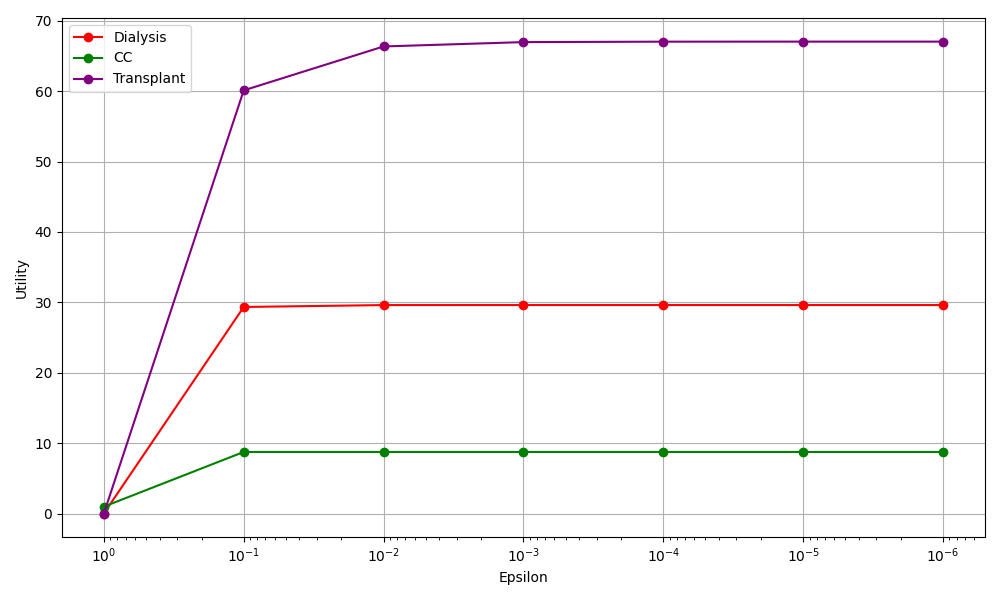
\includegraphics[width=0.95\linewidth]{e_vs_util.png}
  \caption{Utility vs Epsilon}
  \label{fig:utility_vs_epsilon}
\end{figure}

For our value iteration, we used an \(\epsilon\) of \(10E-4\). When choosing an epsilon value it is crucial to not choose a value that is too low. As shown in Figure \ref{fig:utility_vs_epsilon}, at low values of \(\epsilon\), the reward values become linear. Therefore, our choice of \(\epsilon\) was small enough not to impact the results in a significant way.

\begin{figure}[H]
  \centering
  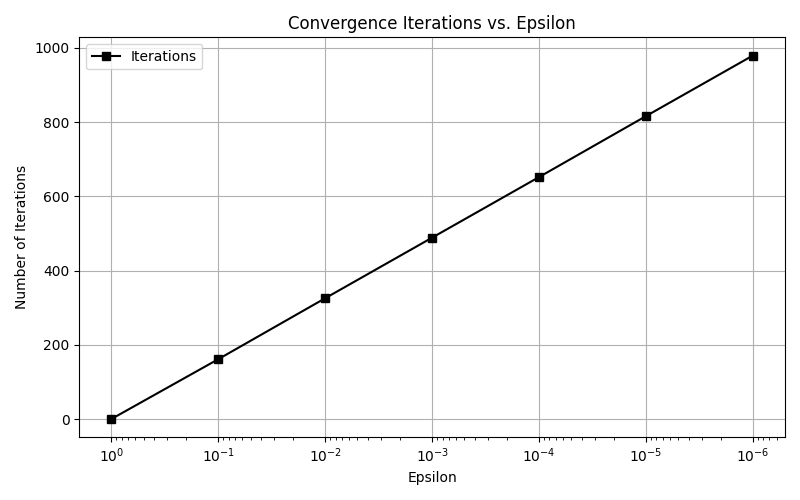
\includegraphics[width=0.95\linewidth]{e_vs_iters_1.png}
  \caption{Iterations vs Epsilon}
  \label{fig:iters_vs_epsilon}
\end{figure}

Figure \ref{fig:iters_vs_epsilon} shows the number of iterations vs the choice of epsilon, and, interestingly, there is a linear relationship between the two. Proof as to why this is the case can be found in \cite{ai}. There were very small differences in reward values as the iterations increased above a certain threshold.

\subsection{Monte Carlo}

We also ran a Monte Carlo simulation with \(N = 100,000\). This choice of \(N\) was large enough to provide accurate results, but not so big that it took an unreasonable amount of time. The Monte Carlo simulation was able to provide us with more results than the MDP, which allowed us to better compare the different treatments to each other. Again, the following tables are in months, except for the QALY table.

\begin{center}
  \begin{tabularx}{\columnwidth}{X c c}   \toprule
  \textbf{Decision} & \textbf{Lifespan (Mean)} & \textbf{Lifespan (SD)} \\
  \midrule
 CC & 10.164369 & 9.566915 \\
 Dialysis, Fistula & 50.832281 & 50.297105 \\
 Dialysis, No Fistula & 45.413938 & 45.875516 \\
 Transplant & 109.760794 & 112.305906 \\
 Transplant, Fistula & 162.093939 & 122.189669 \\
 Transplant, No Fistula & 156.330637 & 118.209652 \\
  \bottomrule
  \end{tabularx}
  \captionof{table}{Lifespan results from simulation with 100{,}000 samples. }
  \label{tab:2}
\end{center}

The first four decisions listed in table \ref{tab:2} correspond to the decisions present in the MDP. Here we see that the lifespan of individuals who chose transplant is greatest at 110 months, with CC the lowest at a little over 10 months. In terms of dialysis with a fistula vs without, it seems that a fistula increased one's lifespan by about 6 months, a significant amount. Finally, the last two columns of the model, represent those individuals who were given a transplant and then had it fail and were then put on dialysis. The life span of these patients being higher makes sense, because in transplant only, you either keep living with it or die. The patients who had a transplant and then dialysis are the ones who did not die while on their transplant and continued living with dialysis. Lifespan was not a measure we could calculate using the MDP, so there are no comparisons that can be made between the two models.


\begin{center}
  \begin{tabularx}{\columnwidth}{X c c} 
  \toprule
  \textbf{Decision} & \textbf{QoL (Mean)} & \textbf{QoL (SD)} \\
  \midrule
 CC & 0.726293 & 0.272583 \\
 Dialysis, Fistula & 0.774744 & 0.130685 \\
 Dialysis, OneMonth & 0.707516 & 0.170910 \\
 Transplant & 0.887768 & 0.162923 \\
 Transplant, Fistula & 0.897094 & 0.035479 \\
 Transplant, OneMonth & 0.882115 & 0.047723 \\
  \bottomrule
  \end{tabularx}
  \captionof{table}{Quality of Life results from simulation with 100{,}000 samples.}
  \label{tab:1}
\end{center}

Table \ref{tab:1} represents the average quality of life of a patient for each treatment. As we can see, transplant has the highest quality of life, followed by dialysis and then CC. Furthermore, given one is on dialysis, it is best to choose dialysis with the fistula, as it offers almost a 0.07 higher QoL. These results make sense, because with a transplant there is the initial discomfort of surgery, but then the QoL is high, the symptoms of the disease are lowered and the patient only has to take some immunosuppressants. Dialysis is lower than transplant, which makes sense because the dialysis procedure hinders daily life and while it can be done at home many patients go to specific centers for dialysis. These sessions can be a few times a week and can last for several hours. Finally, intuitively, one would think that CC should have the highest QoL because a patient does not have to get surgery or dialysis. However, generally, during CC the kidney's functions aren't being replaced, which often leads to higher side-effects of the disease and worsening symptoms, which makes it hard to live a completely healthy life. Again, given that you had a transplant and your kidney failed or was rejected, it is best to go back onto dialysis with a fistula, but only by a very small QoL gain, about 0.015, which for some patients may not be worth the additional surgery.


\begin{center}
  \begin{tabularx}{\columnwidth}{X c c} 
  \toprule
  \textbf{Decision} & \textbf{QALY} \\
  \midrule
 CC & 0.615192 \\
 Dialysis, Fistula & 3.281833 \\
 Dialysis, OneMonth & 2.677592 \\
 Transplant & 8.120172 \\
 Transplant, Fistula & 12.117785 \\
 Transplant, OneMonth & 11.491801 \\
  \bottomrule
  \end{tabularx}
  \captionof{table}{Quality-adjusted life years (QALY) results from simulation with 100{,}000 samples.}
\end{center}

Finally, we can combine the results from the QoL and life-span measurements to get the Quality Adjusted Life Years (QALY). Specifically, QALY is defined by the formula below, meaning that we have to convert the calculated values from per month to per year.

\begin{equation*}
 \text{QALY} = \frac{\mu_{\text{months}} \times \mu_{\text{QoL}}}{12}
\end{equation*}    

Here the \(\mu_{\text{months}}\) is the average quality of life and \(\mu_{\text{QoL}}\) is the lifespan. From the results in the table above, it is clear that the greatest quality of life results from choosing the treatment transplant. We see it is about 4.83 QALY more than on dialysis with a fistula, and about 7.5 QALY more than on CC. Furthermore, it is again the case that fistula does better than not when one goes to dialysis after a transplant, with an increase of about 0.63 years. These results make sense, as patients who do not opt for kidney replacement therapy generally do not live long with CKD five, and those who get a transplant survive significantly longer and have better QoL than those who are just on dialysis, whether with fistula or not.

\begin{figure}[H]
  \centering
  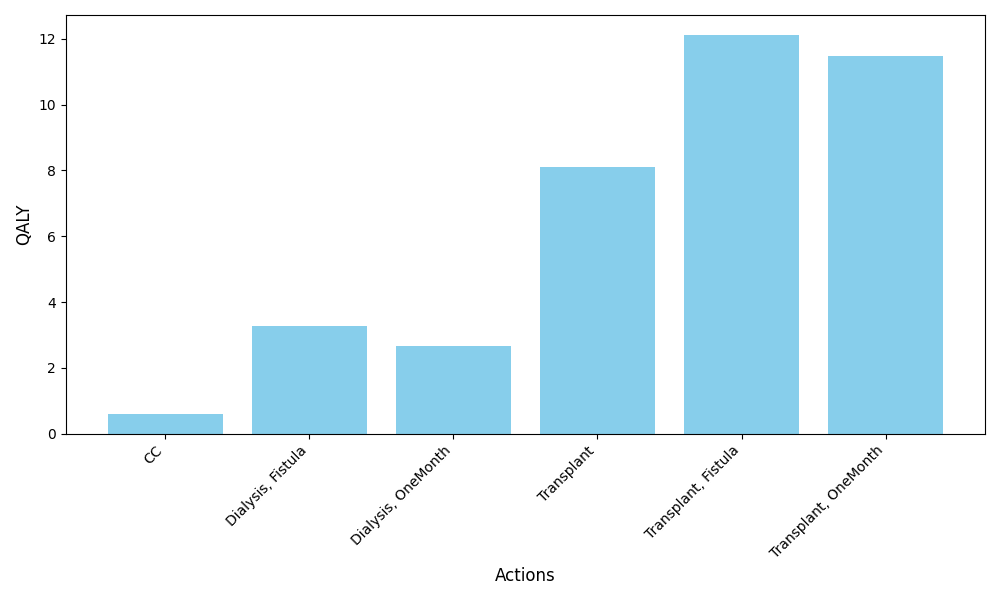
\includegraphics[width=0.95\linewidth]{actions_vs_qaly.png}
  \caption{QALY values for Different Actions}
  \label{fig:1}
\end{figure}

Figure \ref{fig:1} is helpful for visualizing the increased benefit each action has on QALY. It is important to note that in this study, all patients are assumed to be able to receive any treatment. However, many people, may not qualify for a transplant or not be able to find a matching donor kidney in time.

\begin{figure}[H]
  \centering
  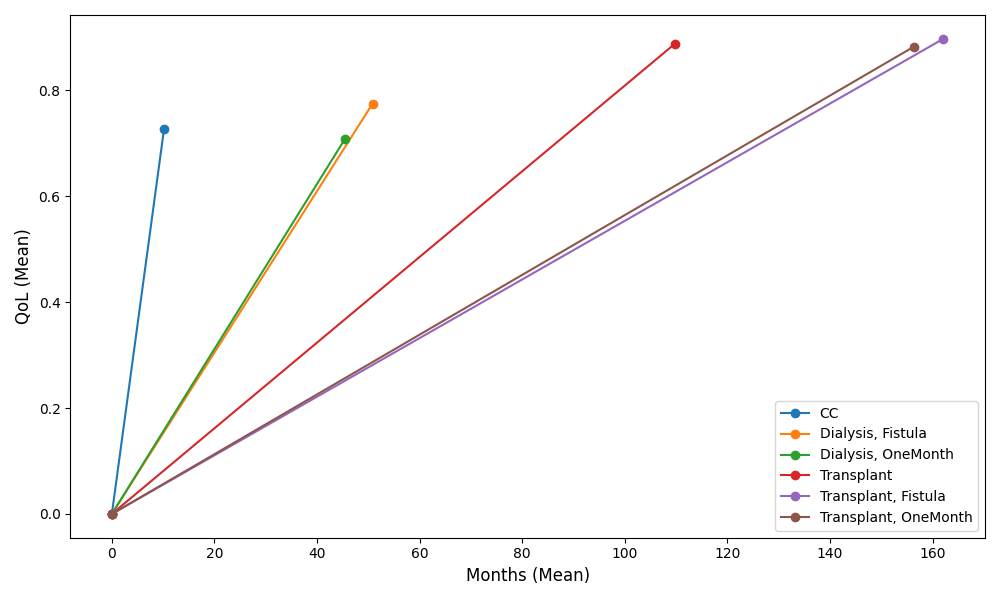
\includegraphics[width=0.95\linewidth]{months_vs_qol.png}
  \caption{QoL vs Months for Different Actions}
  \label{fig:2}
\end{figure}

Figure \ref{fig:2} shows QoL vs the lifespan of an individual. This is just another way to represent QALY. We can see how CC has a fairly high QoL, but a very short lifespan, resulting in its low QALY. The graph shows us that CC has the largest slope, meaning that in the short term one will expect the greatest QoL from choosing the treatment CC. The model rewards living longer, but some patients may prioritize short-term QoL over long-term QALY. If we wanted to model this, we could add in a discount rate, similar to the \(\gamma\) value in method 1, which may alter our results slightly, depending on the value of \(\gamma\). However, most patients, care about both QoL and lifespan, making QALY the most widely used measure for measuring the effectiveness of a treatment.\\

\subsection{Model Comparison}
The values calculated during value iteration should represent the expected utilities of each action, which should closely correlate with the QoL measurement. In fact, it is very surprising that the values are so different. In the adjusted column of figure \ref{tab:here}, we normalized the reward column, with the greatest value, which is of transplant, being the same as the calculated value for transplant from the Monte Carlo results. As you can see the results are decently far off from each other. Specifically, the values for each of the treatments transplant, CC, and Dialysis, are farther spread apart in the value iteration approach than in the Monte Carlo simulation.
Despite the differences, the final conclusions are still the same, and as discussed, MDPs does not necessarily need the most accurate transition values to reach the optimal policy. 

However, I believe the explanation for why these results are not similar lies in the way the models were solved, specifically the way time was treated. When doing value iteration, at each cycle through all the states, each death state is forwarding its 0.0 value. However, in the Monte Carlo simulation, the simulation stops once an individual reaches the death state. This means that the value iteration solution is looking more at a fixed time period, where it measures the average QoL over the entire period, even if a person is dead for most of the period. Meanwhile, in the Monte Carlo simulation, there is no fixed time period resulting, meaning that the time period is the individual's lifespan, not a fixed number of years. I believe that if one were to fix the number of years, we would get results from the value iteration method that is very similar to the Monte Carlo solution. Regardless, both models agree with each other on what the best actions are.

% ------------------------------------------------------------------------------------------
%    Conclusion
% ------------------------------------------------------------------------------------------
\section{Conclusion}

This paper examined which treatment for patients with CKD5 is best. We used a MDP to model the progression of the disease and the complications that occur in patients randomly. We solved the MDP using value iteration, which gave us the optimal policy. From the policy, we determined a transplant is the best option, followed by dialysis and finally CC. Furthermore, we found that if a patient decides to be on dialysis, they should opt for the fistula. We then solved the model using Monte Carlo simulation and determined the mean lifespan, QoL, and QALY for each of the possible actions. Finally, we compared the results of our two approaches and saw that they agreed on which actions were best. Further work could be done to add more complexity to the model. In addition, parameter sensitivity for the model could be tested. Also, the discount factor \(\gamma\) could be used to simulate patients who prefer short-term QoL over long-term QALY.

\pagebreak
\nocite{*}
\bibliographystyle{plain}
\bibliography{final_paper}

\pagebreak

\appendix
\section*{Appendix: Code Listing}

\onecolumn
\allowbreak
\begin{lstlisting}[language=Python]
 """
 This file contains the MDP model that was used. These constants are 
 used for both methods.
 """
  
 states = [
 "CKD5",
 "A_CC",
 "A_Dialysis",
 "A_Transplant",
 "CC",
 "Dialysis",
 "Transplant",
 "Death",
 "Stroke",
 "Disability",
 "MI",
 "CHF",
 "A_Fistula",
 "A_OneMonth",
 "Fistula",
 "OneMonth",
 "AfterOneMonth",
 "Successful",
 "Stroke_D",
 "Disability_D",
 "MI_D",
 "CHF_D",
 "Stroke_DA",
 "Disability_DA",
 "MI_DA",
 "CHF_DA",
 "Stroke_T",
 "Disability_T",
 "MI_T",
 "CHF_T",
 "Stroke_F",
 "Disability_F",
 "MI_F",
 "CHF_F",
 ]
  
 actions = {
 "CKD5": ["A_CC", "A_Dialysis", "A_Transplant"],
 "Dialysis": ["A_Fistula", "A_OneMonth"],
 }
  
 utilities = {
 "CC": 0.98,
 "Fistula": 0.85,
 "Death": 0.0,
 "OneMonth": 0.8,
 "AfterOneMonth": 0.8,
 "Successful": 0.95,
 "Disability": 0.35,
 "Disability_F": 0.35,
 "Disability_D": 0.35,
 "Disability_DA": 0.35,
 "Disability_T": 0.35,
 "CHF": 0.76,
 "CHF_F": 0.76,
 "CHF_D": 0.76,
 "CHF_DA": 0.76,
 "CHF_T": 0.76,
 "Stroke": 0.5,
 "Stroke_F": 0.5,
 "Stroke_D": 0.5,
 "Stroke_DA": 0.5,
 "Stroke_T": 0.5,
 "MI": 0.5,
 "MI_F": 0.5,
 "MI_D": 0.5,
 "MI_DA": 0.5,
 "MI_T": 0.5,
 }
  
 transitions = {
 # CC subtree
 "CC": [("Death", 0.09812), ("Stroke", 0.006), ("MI", 0.00792), ("CC", 0.88796)],
 "Stroke": [("Disability", 0.33), ("Death", 0.2), ("CC", 0.47)],
 "MI": [("Death", 0.08), ("CHF", 0.05), ("CC", 0.87)],
 "Disability": [("CC", 1.0)],
 "CHF": [("CC", 1)],
 # Transplant subtree
 "Transplant": [("Death", 0.012), ("Successful", 0.988)],
 "Successful": [
 ("Dialysis", 0.0051),
 ("MI_T", 0.0028),
 ("Death", 0.0031),
 ("Stroke_T", 0.003),
 ("Successful", 0.986),
 ],
 "Stroke_T": [("Disability_T", 0.33), ("Death", 0.2), ("Successful", 0.47)],
 "MI_T": [("CHF_T", 0.05), ("Death", 0.08), ("Successful", 0.87)],
 "CHF_T": [("Successful", 1.0)],
 "Disability_T": [("Successful", 1.0)],
 # Fistula subtree
 "Fistula": [
 ("Death", 0.0133),
 ("Stroke_F", 0.0115),
 ("Fistula", 0.9713),
 ("MI_F", 0.0039),
 ],
 "Stroke_F": [("Death", 0.55), ("Disability_F", 0.33), ("Fistula", 0.12)],
 "MI_F": [("Death", 0.08), ("CHF_F", 0.05), ("Fistula", 0.87)],
 "Disability_F": [("Fistula", 1.0)],
 "CHF_F": [("Fistula", 1.0)],
 # OneMonth subtree
 "OneMonth": [
 ("Stroke_D", 0.0115),
 ("Death", 0.0425),
 ("MI_D", 0.0039),
 ("AfterOneMonth", 0.9421),
 ],
 "Stroke_D": [("Disability_D", 0.33), ("Death", 0.492), ("AfterOneMonth", 0.178)],
 "MI_D": [("Death", 0.08), ("CHF_D", 0.05), ("AfterOneMonth", 0.87)],
 "Disability_D": [("AfterOneMonth", 1.0)],
 "CHF_D": [("AfterOneMonth", 1.0)],
 "AfterOneMonth": [
 ("AfterOneMonth", 0.9699),
 ("Stroke_DA", 0.0115),
 ("MI_DA", 0.0039),
 ("Death", 0.0147),
 ],
 "Stroke_DA": [("Death", 0.55), ("Disability_DA", 0.33), ("AfterOneMonth", 0.12)],
 "MI_DA": [("Death", 0.08), ("CHF", 0.05), ("AfterOneMonth", 0.87)],
 "CHF_DA": [("AfterOneMonth", 1.0)],
 "Disability_DA": [("AfterOneMonth", 1.0)],
 }
  
\end{lstlisting}

\begin{lstlisting}[language=Python]
 """
 This file contains the code for the Monte Carlo simulation.
 """
  
 from final_code import states, actions, transitions, utilities
 import random
 import pandas as pd
 import matplotlib.pyplot as plt
  
 num_individuals = 100000
 start_state = "CKD5"
 results = []
  
 for i in range(num_individuals):
 current_state = start_state
 months = 0
 choices = []
 Qol = 0.0
 while current_state != "Death":
 if current_state in actions:
 current_state = random.choice(actions[current_state])[2:]
 choices.append(current_state)
  
 else:
 previous_state = current_state
 next_states, next_probs = list(zip(*transitions[current_state]))
 current_state = random.choices(next_states, weights=next_probs, k=1)[0]
 if current_state in utilities:
 Qol += utilities[current_state]
 months += 1
 results.append((choices, months, Qol / months))
  
 df = pd.DataFrame(results, columns=["actions", "months", "QoL"])
  
 df["action_combined"] = df["actions"].apply(lambda x: ", ".join(x))
 grouped_stats = df.groupby("action_combined")[["months", "QoL"]].agg(["mean", "std"])
 grouped_stats["QALY"] = (
 grouped_stats[("months", "mean")] * grouped_stats[("QoL", "mean")] / 12
 )
 print(grouped_stats)
 print(grouped_stats["QALY"])
  
 # plots
 actions = grouped_stats.index
 qaly_values = grouped_stats[("QALY")].values
 months_values = grouped_stats[("months", "mean")].values
 qol_values = grouped_stats[("QoL", "mean")].values
  
 plt.figure(figsize=(10, 6))
 plt.bar(actions, qaly_values, color="skyblue")
 plt.xlabel("Actions", fontsize=12)
 plt.ylabel("QALY", fontsize=12)
 plt.xticks(rotation=45, ha="right")
 plt.show()
 plt.figure(figsize=(10, 6))
 for i in range(len(actions)):
 plt.plot([0, months_values[i]], [0, qol_values[i]], label=actions[i], marker="o")
 plt.xlabel("Months (Mean)", fontsize=12)
 plt.ylabel("QoL (Mean)", fontsize=12)
 plt.legend()
 plt.show()  
\end{lstlisting}

\begin{lstlisting}[language=Python]
 """
 This file contains the code that was used to determine the effect of
 different epsilon values on the utilities. Most of the code is identical
 to the code in val_iter.py
 """
  
 from final_code import states, actions, transitions, utilities
 import matplotlib.pyplot as plt
  
 eps_val = [10e-1, 10e-2, 10e-3, 10e-4, 10e-5, 10e-6, 10e-7]
 num_iters = []
 utils = []
  
 for e in eps_val:
 V = {state: 0.0 for state in states}
 policy = {state: None for state in states}
 epsilon = e
 iterations = 0
  
 while True:
 iterations += 1
 delta = 0
 new_V = V.copy()
  
 expected_utilities = []
 for state in states:
 state = state[2:] if state.startswith("A_") else state
 list_states = []
 if state in actions:
 best_states = []
 for action in actions[state]:
 action = action[2:]
 best_states.append((V[action], f"A_{action}"))
 list_states.append(max(best_states))
  
 else:
 if state == "Death":
 list_states.append((0.0, "Death"))
 else:
 for s, prob in transitions[state]:
 value = prob * V.get(s, 0.0)
 list_states.append((value, s))
  
 new_val, new_state = max(list_states)
 new_V[state] = utilities.get(state, 0.0) + new_val
 policy[state] = new_state
  
 diff = abs(new_V[state] - V[state])
 delta = diff if delta < diff else delta
 V = new_V
  
 if delta < epsilon:
 break
  
 num_iters.append(iterations)
 utils.append(
 (
 V["CKD5"],
 V["Dialysis"],
 V["CC"],
 V["Transplant"],
 V["Fistula"],
 V["OneMonth"],
 )
 )
  
 print("utils", utils)
 print("ites", num_iters)
  
 plt.figure(figsize=(8, 5))
 plt.plot(
 eps_val, num_iters, marker="s", linestyle="-", color="black", label="Iterations"
 )
 plt.xscale("log")
 plt.gca().invert_xaxis() # so it goes from larger epsilon to smaller epsilon values
 plt.xlabel("Epsilon")
 plt.ylabel("Number of Iterations")
 plt.title("Convergence Iterations vs. Epsilon")
 plt.grid(True)
 plt.legend()
 plt.show()  
\end{lstlisting}

\begin{lstlisting}[language=Python]

"""
This file contains all the code used to compute the value iteration
and to get the optimal policy.
"""

from final_code import states, actions, transitions, utilities

V = {state: 0.0 for state in states}
policy = {state: None for state in states}
epsilon = 1e-4
iterations = 0

while True:
 iterations += 1
 delta = 0
 new_V = V.copy()

 expected_utilities = []
 for state in states:
 state = state[2:] if state.startswith("A_") else state
 list_states = []
 if state in actions:
 best_states = []
 for action in actions[state]:
 action = action[2:]
 best_states.append((V[action], f"A_{action}"))
 list_states.append(max(best_states))

 else:
 if state == "Death":
 list_states.append((0.0, "Death"))
 else:
 for s, prob in transitions[state]:
 value = prob * V.get(s, 0.0)
 list_states.append((value, s))

 new_val, new_state = max(list_states)
 new_V[state] = utilities.get(state, 0.0) + new_val
 policy[state] = new_state

 diff = abs(new_V[state] - V[state])
 delta = diff if delta < diff else delta
 V = new_V

 if delta < epsilon:
 break

utils = [
 V["CKD5"],
 V["Dialysis"],
 V["CC"],
 V["Transplant"],
 V["Fistula"],
 V["OneMonth"],
]


print("V", V)
print("Policy", policy)
print("iterations", iterations)

print("_________________")
print("CKD5", "Dialysis", "CC", "Transplant", "Fistula", "OneMonth")
print(utils)

max_val = max(utils)
normalized_utils = [v / max_val for v in utils]
print(normalized_utils)

target_max = 0.887
max_val = max(utils)
normalized_utils = [v / max_val * target_max for v in utils]
print(normalized_utils)

\end{lstlisting}

\end{document}


% \url{https://www.kidneyfund.org/living-kidney-disease/healthy-eating-activity}
% \url{https://www.cdc.gov/diabetes/diabetes-complications/diabetes-and-chronic-kidney-disease.html#:~:text=Diabetes}
% \url{https://link.springer.com/article/10.1007/s12325-021-02006-z}
% \url{https://www.youtube.com/watch?v=2iF9PRriA7w}
% \url{https://www.kidney.org/kidney-topics/stages-chronic-kidney-disease-ckd}
% \url{https://link.springer.com/chapter/10.1007/978-3-319-43742-2_24?fromPaywallRec=true}
% \url{https://pmc.ncbi.nlm.nih.gov/articles/PMC3132702/}
% \url{https://pmc.ncbi.nlm.nih.gov/articles/PMC6892339/}
% \url{https://pmc.ncbi.nlm.nih.gov/articles/PMC5749372/}
% \url{https://www.cdc.gov/kidney-disease/php/data-research/index.html}


% digraph {
%     CKD5 -> Action_CC
%     CKD5 -> Action_Dialysis
%     CKD5 -> Action_Transplant

%     Action_CC -> CC
%     Action_Dialysis -> Dialysis
%     Action_Transplant -> Transplant

%     CC -> Death [label=0.09812]
%     CC -> Stroke [label=0.006]
%     Stroke -> Death [label=0.2]
%     Stroke -> Disability [label=.33]
%     Disability -> CC [label=1]
%     CC -> MI [label=0.00792]
%     MI -> Death [label=0.08]
%     MI -> CHF [label=0.05]
%     CHF -> CC [label=1]

%     Dialysis -> Action_Catheter
%     Dialysis -> Action_Fistula

%     Action_Catheter -> OneMonth
%     Action_Fistula -> Fistula

%     OneMonth -> Death_D [label=0.0425]
%     OneMonth -> Stroke_D [label=0.0115]
%     Stroke_D -> Death_D [label=.492]
%     Stroke_D -> Disability_D [label=0.33]
%     Disability_D -> AfterOneMonth [label=1]
%     OneMonth -> AfterOneMonth [label=0.9421]
%     OneMonth -> MI_D [label=.0039]

%     AfterOneMonth -> Death_DA [label=0.0147]
%     AfterOneMonth -> Stroke_DA [label=0.0115]
%     Stroke_DA -> Death_DA [label=0.55]
%     AfterOneMonth -> MI_DA [label=.0039]

%     Fistula -> Death_F [label=0.0133]
%     Fistula -> MI_F [label=0.0039]
%     Fistula -> Stroke_F [label=0.0115]
%     Stroke_F -> Death_F [label=.55]

%     Transplant -> Death_T [label=0.012]
%     Transplant -> Successful [label=0.988]
%     Successful -> Death_T [label=0.0031]
%     Successful -> Dialysis [label=0.0051]
%     Successful -> Stroke_T [label=0.003]
%     Stroke_T -> Death_T [label=0.2]
%     Stroke_T -> Disability_T [label=0.33]
%     Successful -> MI_T [label=0.0028]
%     MI_T -> Death_T [label=0.08]
%     MI_T -> CHF_T [label=0.05]

%     CHF_T -> Successful [label=1]
%     Disability_T -> Successful [label=1]
%     Stroke_F -> Disability_F [label=.33]
%     Disability_F -> Fistula [label=1.0]

%     MI_D -> Death_D [label=0.08]
%     MI_D -> CHF_D [label=0.5]
%     CHF_D -> AfterOneMonth [label=1.0] 

%     MI_F -> Death_F [label=0.08]
%     MI_F -> CHF_F [label=0.05]
%     CHF_F -> Fistula [label=1.0] 

%     MI_DA -> Death_DA [label=0.08]
%     MI_DA -> CHF_DA [label=0.05]
%     CHF_DA -> AfterOneMonth [label=1.0] 

%     CC -> CC [label=0.88796]
%     Successful -> Successful [label=0.986]
%     Fistula -> Fistula [label=0.9713]
%     AfterOneMonth -> AfterOneMonth [label=.9699]
%     Stroke_DA -> Disability_DA [label=0.33]
%     Disability_DA -> AfterOneMonth [label=1.0]

%     Stroke -> CC [label=0.47]
%     MI -> CC [label=0.87]
%     Stroke_T -> Successful [label=0.47]
%     MI_T -> Successful [label=0.87]
%     Stroke_F -> Fistula [label=0.12]
%     MI_F -> Fistula [label=0.87]
%     Stroke_D -> AfterOneMonth [label=0.178]
%     MI_D -> AfterOneMonth [label=0.87]
%     Stroke_DA -> AfterOneMonth [label=0.12]
%     MI_DA -> AfterOneMonth [label=0.87]

% }

% \begin{figure*}[ht]
%   \centering
%   \begin{tikzpicture}[->, thick, node distance=4cm, auto]
  
%     \node[draw, rounded corners, minimum width=2.5cm] (s5) {CKD Stage 5};
  
%     \node[draw, below left of=s5, minimum width=2.5cm] (med) {Medication};
%     \node[draw, right of=med, minimum width=2.5cm] (noTx) {No Treatment};
%     \node[draw, right of=noTx, minimum width=2.5cm] (dialysis) {Dialysis};
%     \node[draw, right of=dialysis, node distance=4cm, minimum width=2.5cm] (transplant) {Transplant};
  
%     \node[draw, below of=med, node distance=2cm, minimum width=2.5cm] (bone) {Bone Disease};
%     \node[draw, below of=noTx, node distance=2cm, minimum width=2.5cm] (mi) {MI};
%     \node[draw, below of=dialysis, node distance=2cm, minimum width=2.5cm] (stroke) {Stroke};


%     \node[draw, below right of=mi, node distance=4cm, minimum width=2.5cm] (death) {Death};
  
%     \draw (s5) -- node[left] {C(M)} (med);
%     \draw (s5) -- node[right] {0} (noTx);
%     \draw (s5) -- node[left] {C(D)} (dialysis);
%     \draw (s5) -- node[above] {C(T)} (transplant);
  
%     \draw (med) -- node[left] {} (bone);
%     \draw (noTx) -- node[left] {} (bone);
%     \draw (dialysis) -- node[left] {} (bone);
%     \draw (transplant) -- node[left] {} (bone);

%     \draw (med) -- node[left] {} (mi);
%     \draw (noTx) -- node[left] {} (mi);
%     \draw (dialysis) -- node[left] {} (mi);
%     \draw (transplant) -- node[left] {} (mi);

%     \draw (med) -- node[left] {} (stroke);
%     \draw (noTx) -- node[left] {} (stroke);
%     \draw (dialysis) -- node[left] {} (stroke);

%     \draw (med) -- node[left] {} (death);
%     \draw (noTx) -- node[left] {} (death);
%     \draw (dialysis) -- node[left] {} (death);
%     \draw (transplant) -- node[left] {} (death);
  
%   \end{tikzpicture}
%   \caption{CKD Stage 5 model}
%   \label{fig:ckd-simple-graph}
%   \end{figure*}